\subsection{Methodology}
This project lends itself to being suitable for an agile development methodology, given that it is small with a single inexperienced developer, requirements and time constraints may change, and having frequent builds with new progress ensures that some functioning product will exist by the end. Sprints will range from 1-3 weeks long depending on the size of the feature(s) being implemented in that sprint, and the time available to work on the project during the sprint.

\subsection{Timetable}
% Gantt image
\begin{figure}[h!]
    \centering
	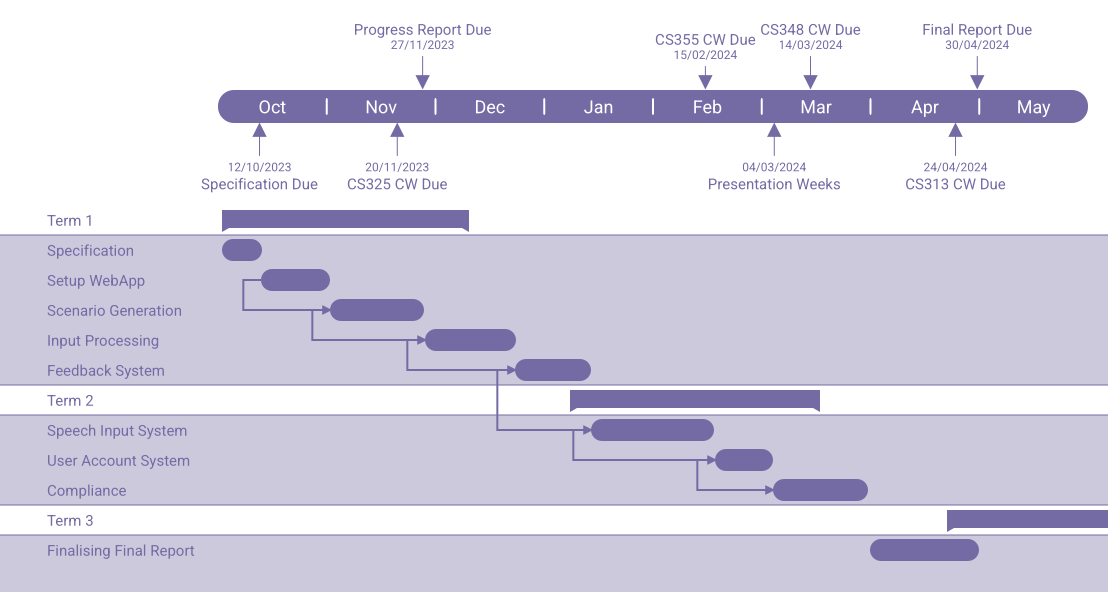
\includegraphics[scale = 0.42]{../document-resources/images/initial-gantt.png}
    \label{initialgantt}
    \caption{Proposed project timeline}
\end{figure}

\subsection{Risk Assessment}
The risks involved in this project are primarily related to the people and technologies required to build it.
The technology risks include access to the APIs that will be relied upon to obtain data which I cannot feasibly obtain myself within the scope of the project.
At any time the APIs could be changed or removed, which would require a change in the project scope, but can be somewhat mitigated by keeping features modular, so that they can be removed or replaced with minimal impact on the rest of the system.
The Google Maps API is free for \$200 worth of transactions per month, which should be sufficient for the project. However, it is possible that this limit be reached, which would require reconsidering the use of the API.
The Bing Maps API currently is free for educational use with a limit of 125,000 transactions per year, which could be used as a backup if limits are exceeded on the Google Maps API.
\subsection{Resources}
All project code and documents will be stored in a GitHub repository with a CI\textbackslash CD set up in GitHub Actions to ensure the latest production version is always hosted via GitHub Pages. Online hosted version control ensures that access to the codebase and documents is simple and always available, and that mistakes can be reverted if needed. CI\textbackslash CD ensures that a testable version of the project is available at all times so feedback can be gained more often and on a recent version and no extra effort will be required to create a functioning prototype for the presentation.
% Languages used
% Libraries used
% David?
% APIs used
\subsection{Legal, Social, Ethical, Professional Issues and Concerns}
Given that the target users of the system will mainly be trainee pilots, it is paramount that the information taught by the system follows the guidelines set by the UK Civil Aviation Agency (CAA). Incorrect teaching could be a factor in an incident if proper 